
% ----------------------------------------------------------
% CAPÍTULO 03 - METODOLOGIA E DADOS
% ----------------------------------------------------------

\chapter{Metodologia e dados} \label{cha:metodologia}

Este capítulo descreve os modelos de Equilíbrio Geral Computável e microssimulação comportamental utilizados para estimar os efeitos do comércio internacional sobre a distribuição da renda familiar e os níveis de pobreza no Brasil. Também se apresenta a base de dados usada para a calibragem dos referidos modelos e a implementação da estratégia empírica para simular os efeitos de um choque de liberalização comercial.


\section{O modelo de Equilíbrio Geral Computável} \label{sec:egc}

Utiliza-se o modelo nacional estático de Equilíbrio Geral Computável para o Brasil, o ORANIG-BR, adaptado para cumprir os objetivos propostos nesta dissertação. Esse modelo partiu da estrutura teórica do ORANI \cite{dixit80}, de tradição australiana do tipo Johansen\footnote{Caracteriza-se por ter um escopo matemático concebido a partir de um conjunto de equações linearizadas e as soluções são apresentadas como elasticidades, representando as taxas de crescimento, sendo possível diversos tipos de fechamento.}.

Sua especificação teórica é composta por blocos de equações que determinam as relações de oferta a partir das hipóteses de otimização e \textit{market clearing}. O modelo incorpora os pressupostos neoclássicos das firmas minimizadoras de custos, famílias maximizadoras de utilidade e equilíbrio dos mercados - esta sendo garantida desde que a oferta e demanda se igualem para o mercado de produtos e serviços domésticos, importados, margens e para o mercado de trabalho.

O uso do modelo de EGC para estudos de análise política, sobretudo sobre impactos e efeitos de algum determinado fenômeno econômico, político ou histórico se tornou cada vez mais frequente na literatura econômica. Há diversos benefícios em trabalhar com esse modelo: é possível operar com altos níveis de desagregação setorial e regional; considerar as relações de interdependência entre os setores e os agentes econômicos; e capturar o efeito-renda e efeito-preço, que estão diretamente relacionados com os canais de transmissão entre comércio internacional e desigualdade de renda e pobreza \cite{anderson20}.

Para esta dissertação, foram realizadas três principais modificações no modelo ORANIG-BR: 1- o fator trabalho foi dividido em três categorias que refletem os diferentes tipos de força de trabalho a partir do nível de escolaridade; 2- as famílias foram divididas em cem categorias de acordo com a renda; e 3- o fluxo das exportações foi dividido entre vinte e seis parceiros comerciais. A Figura~\ref{fig:estrutura_orani} apresenta a estrutura esquemática do modelo ORANIG-BR com as referidas modificações e a Figura~\ref{fig:dados_orani} apresenta a base de dados.


\begin{landscape}
	\begin{figure}
		\centering
		\caption{Representação esquemática do modelo ORANIG-BR} \label{fig:estrutura_orani}
		
\includegraphics[width=0.95\linewidth]{Imagens/002.ai}
		\footnotesize \\
		Fonte: elaboração própria (2024) a partir de \textcite{souza15}
	\end{figure}
\end{landscape}

\begin{figure}[H]
	\centering
	\caption{Base de dados do modelo ORANIG-BR} \label{fig:dados_orani}
	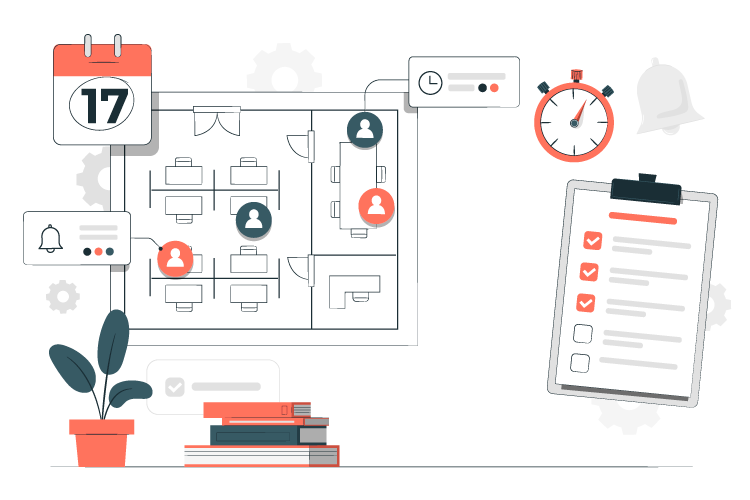
\includegraphics[width=\textwidth]{Imagens/003.ai}
	\footnotesize
	Fonte: elaboração própria (2024) a partir de \textcite{horridge00}
\end{figure}


\subsection{Produção} \label{subsec:producao}

Os setores produtivos seguem os pressupostos neoclássicos de minimização dos custos numa estrutura de mercado de concorrência perfeita, sujeitos a tecnologias de retornos constantes de escala - representadas por funções CES e Leontief. A Figura \ref{fig:estrutura_producao} apresenta a estrutura de produção do modelo. Há cerca de três produtos: 1- bens intermediários; 2- fatores primários; e 3- outros fatores\footnote{"Outros fatores" são as taxas e subsídios do modelo.}. Para se produzir o primeiro, deve-se combinar uma determinada composição das \textit{commodities} disponíveis, decidindo sua origem - se doméstico ou importado. Para produzir o segundo, deve-se combinar quantidades relativas de capital e trabalho, sendo que este é determinado a partir de uma combinação dos três tipos disponíveis de trabalhadores.

Desse modo, para poder produzir nesse modelo, deve-se combinar os bens intermediários, os fatores primários e os outros fatores a partir da minimização dos custos da função Leontief\footnote{Isso implica que esses três fatores são complementares perfeitos, não admitindo substituição}.

\begin{align}
	\underset{i = 1, ... , 124}{Leontief} \{\frac{X_{ij}}{A_{ij}}\} = A_jZ_j, \hspace{2cm} j = 1, ... , 65
\end{align}

No qual $X_{ij}$ corresponde ao insumo $i$ da indústria $j$; $Z_j$ é o nível de atividade da indústria $j$; e $A_ij$ é o coeficiente tecnológico. Se este é igual a 1, significa que é o coeficiente insumo-produto que mostra o insumo mínimo efetivo de $i$ necessário para sustentar uma unidade de atividade na indústria $j$ \cite{dixit80}.

A decisão entre a fonte doméstica ou importada é modelada a partir da hipótese de \textcite{armington69} a qual relaciona os insumos de ambas as fontes como substitutos imperfeitos. Desse modo, para capturar esse efeito, assume-se as unidades de um determinado insumo, diferenciáveis apenas pela fonte, são combinadas para fornecer um só insumo, chamado de \textit{insumo efetivo}:

\begin{align}
	X_{ij} = \underset{s = 1, 2}{CES} = \{\frac{X_{(is)j}}{A_{(is)j}}; \rho_{ij}, b_{(is)j}\}, \hspace{2cm} i & = 1, ... , 124 \\ j & = 1, ... , 65 \notag
\end{align}

No qual $X_{(is)j}$ se refere ao insumo $i$ da fonte $s$ pertencente ao setor $j$; $\rho$ e $b$ são parâmetros de substituição entre as variáveis doméstica e importada. 

\begin{landscape}
	\begin{figure}
		\centering
		\caption{Estrutura de produção do modelo ORANIG-BR} \label{fig:estrutura_producao}
		\includegraphics[width=0.9\linewidth]{Imagens/004.ai}
		\footnotesize \\
		Fonte: elaboração própria (2024) a partir de \textcite{horridge00}
	\end{figure}
\end{landscape}

\subsubsection{Composição do fator trabalho} \label{}

Como dito anteriormente, o fator trabalho foi subdividido em três grupos: não qualificado, semi-qualificado e qualificado. Esta divisão segue a intuição de que os produtores buscam um determinado conjunto de habilidades no mercado de trabalho que melhor se adeque a demanda do setor produtivo.

Essa habilidade é representada por anos de educação. O Quadro \ref{quad:categoria_trabalho} apresenta a categorização escolhida para desagregar o fator trabalho.

\begin{quadro}[h]
	\centering
	\begin{threeparttable}
		\caption{Categorização do fator trabalho} \label{quad:categoria_trabalho}
		\footnotesize
		\begin{tabular}{|| m{3cm} | m{9cm} ||}
			\hline \hline
			\multicolumn{1}{||c|}{\textbf{variável}} & \multicolumn{1}{c||}{\textbf{descrição}} \\ \hline
			não qualificado  & até Ensino Fundamental completo (até onze anos de estudo) \\ \hline 
			semi-qualificado & até Ensino Médio completo (doze a quinze anos de estudo) \\ \hline
			qualificado      & Ensino Superior (dezesseis anos ou mais de estudo) \\ \hline \hline
		\end{tabular}
		\begin{tablenotes}
			\scriptsize
			\item Fonte: elaboração própria (2024) a partir do \textcite{inep04}
		\end{tablenotes}
	\end{threeparttable}
\end{quadro}

\subsection{Demanda das famílias} \label{subsec:demanda_familias}



A demanda é composta por cem famílias representativas, distribuídas por percentis da renda total. Cada família determina uma composição ótima de sua cesta de consumo, escolhendo os insumos de tal maneira a maximizar uma função de utilidade Klein-Rubin sujeita a restrição do orçamento familiar \cite{horridge03}. A Figura \ref{fig:estrutura_familia} apresenta a estrutura da demanda das famílias no modelo ORANIG-BR.

A função Klein-Rubin é não-homotética; ou seja, o aumento da renda altera as participações orçamentárias, mesmo com taxas de preço fixas. O consumo é dividido entre dois bens, "subsistência" e "luxo", de tal maneira que o primeiro detém um consumo fixo e o segundo, residual. Diferentemente da função Leontief, a composição das \textit{commodities} é dado por um LES \cite{horridge03}.

Nesse sistema, participação do gasto acima do nível de subsistência, para cada bem, representa uma proporção constante do gasto total de subsistência de cada família representativa. A função de utilidade é dada por:

\begin{align*}
	U(\bar{X}_1, ... , \bar{X}_{124})
\end{align*}

Sujeito a:

\begin{align}
	&\bar{X}_i = \underset{s = 1, 2}{CES} (\bar{X}_{(is)}), \hspace{2cm} i = 1, ... , 124 \\
	&\sum_{s = 1}^{2} \sum_{i = 1}^{124} \bar{P}_{(is)} \bar{X}_{(is)} = C
\end{align}

\begin{landscape}
	\begin{figure}
		\centering
		\caption{Estrutura da demanda das famílias do modelo ORANIG-BR} \label{fig:estrutura_familia}
		\includegraphics[width=0.6\linewidth]{Imagens/005.ai}
		\footnotesize \\
		Fonte: elaboração própria (2024) a partir de \textcite{horridge00}
	\end{figure}
\end{landscape}

\subsection{Fechamento do modelo} \label{subsec:fechamento}

Utiliza-se a versão estática do modelo ORANIG-BR porque as vantagens da dinâmica recursiva não seriam aproveitadas neste exercício empírico. O efeito da estrutura produtiva e da distribuição funcional da renda composição que se espera observar pode ser integralmente captado em um modelo estático.

A Figura~\ref{quad:fechamento} apresenta o fechamento de curto-prazo adotado no modelo, seguindo as especificações de \textcite{horridge03}. Ou seja, tornou-se exógeno: 1- as variáveis do PIB real - exceto a balança comercial; os fatores produtivos; e 3- as taxas de impostos e distribuição dos investimentos entre as indústrias.

Esse fechamento emula o seguinte comportamento econômico. No curto-prazo, o estoque de capital, a tecnologia e o salário real são exógenos. Isso permite ao modelo determinar o emprego real e, consequentemente, o PIB real. Pelo fato do PIB ser determinado pelo lado da oferta, tendo sua absorção doméstica praticamente formada, a balança comercial, no curto-prazo, ganha a função de ser uma variável de ajuste para a identidade do PIB. Ou seja, o movimento do PIB é determinado pelo movimento da balança comercial.

A lista com todas as variáveis exógenas do modelo se encontra no Apêndice~\ref{ap:a}.


\begin{quadro}[h]
	\centering
	\begin{threeparttable}
		\caption{Variáveis de \textit{swap} no fechamento de curto-prazo} \label{quad:fechamento}
		\footnotesize
		\begin{tabular}{||l m{6.5cm} |l m{5.5cm} ||}
			\hline \hline
			\multicolumn{2}{||c|}{\textbf{Antiga exógena}}                     & \multicolumn{2}{c||}{\textbf{Nova exógena}} \\ \hline
			\textbf{Variáveis} & \multicolumn{1}{c|}{\textbf{Descrição}}      & \textbf{Variáveis} & \multicolumn{1}{c||}{\textbf{Descrição}} \\ \hline
			\textit{f1lab\_io}  & mudança geral dos salários                  & \textit{realwage}  & salário real \\
			\textit{x2tot}     & investimento setorial                        & \textit{finv1}     & deslocamento da regra de investimento \\
			\textit{f5tot2}    & desloc. entre demandas do governo e famílias & \textit{x5tot}     & demanda agregada do governo \\
			\textit{invslack}  & var. para tornar o invest. agregado exógeno  & \textit{x2tot\_i}  & investimento agregado por setor \\ \hline \hline
		\end{tabular}
		\begin{tablenotes}
			\scriptsize
			\item Fonte: elaboração própria (2024)
		\end{tablenotes}
	\end{threeparttable}
\end{quadro}


\section{Base de dados e calibragem} \label{sec:dados_egc}

A base de dados do modelo foi calibrada a partir da Matriz de Insumo-Produto do \Citetitle*{scn} do Instituto Brasileiro de Geografia e Estatística (IBGE), contendo 128 produtos e 68 setores econômicos para o ano de 2015. Para esta dissertação, os setores foram agregados em 65 atividades econômicas que produzem 124 produtos. O modelo conta com 114 componentes da demanda final (cem famílias, governo, investimento, exportações e estoque), dois fatores primários (capital e trabalho agregado), três tipos de trabalho (não qualificado, semi-qualificado e qualificado), dois setores de margens (comércio e transporte), e importações por produto para cada um dos 124 produtos.

Para desagregar o fator trabalho e detalhar as famílias em cem classes divididas por percecntis de renda total familiar, utilizou-se, respectivamente, os dados da \Citetitle*{pnad}, do ano de 2015, e da \Citetitle*{pof}, do ano 2008-2009, ambos do IBGE. A escolha por essas edições da PNAD e POF, e não uma mais recente, foi motivada pelo fato do modelo ORANIG-BR ter sido calibrado com os dados desses anos.



\section{Modelo de microssimulação} \label{sec:microssimulacao}

Como discutido anteriormente, os modelos de equilíbrio geral são utilizados para capturar os efeitos setoriais de variações nos preços relativos e emprego, permitindo focar nos grupos beneficiados e prejudicados a partir de choques exógenos que simulem políticas comerciais, econômicas ou eventos históricos. Entretanto, não são uma ferramenta adequada para realizar análises distributivas dada a falta de resultados a nível individual \cite{tiberti17}.

Essa limitação está diretamente associada ao pressuposto da Família Representativa\footnote{Nos modelos EGC, o agrupamento familiar é um agregado familiar e não um agregado familiar médio \cite{tiberti17}.} dos modelos de equilíbrio geral. Isso implica que o modelo deve assumir uma distribuição relativa de renda intra-grupo constante para todos. A evidência empírica mostra que componente intra-grupo das mudanças observadas na distribuição de renda é, pelo menos, tão importante quanto o componente entre grupos dessas mudanças \cite{colombo08}.

Por essa razão, os modelos de equilíbrio geral, ao não conseguirem captar esses efeitos a nível microeconômico, podem gerar resultados errôneos - sobretudo se tratando de estudos sobre pobreza. Ao não conseguir capturar a heterogeneidade de uma família, o pressuposto da Família Representativa pode acabar por subestimar o efeito dos choques exógenos \cite{colombo08}. 

Uma alternativa é utilizar os modelos de microssimulação integrados ao modelo de equilíbrio geral. Essa combinação é particularmente útil para estudos sobre desigualdade e pobreza em países em desenvolvimento, uma vez que que tanto o foco micro quanto macroeconômico é requerido: o primeiro para ter um cenário detalhado das rendas e despesas a nível individual, além das reações dos indivíduos frente a choques e outras políticas econômicas; o segundo para poder simular os efeitos diretos e indiretos desses choques sobre toda a estrutura econômica \cite{tiberti17, klevmarken22}.

O modelo de microssimulação pode ser entendido enquanto uma grande variedade de técnicas de modelagem por meio das quais o comportamento ou estado dos indivíduos são estimados ou determinados \cite{figari15}. Em geral, é um modelo sobre o comportamento dos agentes econômicos -- sejam indivíduos, firmas ou famílias. Através dele, é possível estimar os efeitos de políticas econômicas ou quaisquer outros tipos de choque sobre esses agentes.

As microssimulações podem ser paramétricas ou não-paramétricas. A primeira consiste em um sistema de equações que determina um conjunto de comportamentos individuais, como, por exemplo, a decisão de ingressar no mercado de trabalho e a magnitude do retorno do fator trabalho e capital humano. A segunda acontece a partir de um procedimento de seleção aleatória que agrupa indivíduos com características semelhantes a fim de simular certas mudanças \cite{tiberti17m}. Os modelos também podem ser determinísticos ou estocásticos -- comumente chamados na literatura de comportamentais. A diferença reside, respectivamente, na ausência (ou presença) de estimações econométricas sobre o comportamento dos indivíduos.

É interessante integrar o modelo EGC com uma microssimulação porque esses modelos acabam por corrigir suas limitações. Ao passo em que a microssimulação permite analisar os efeitos distributivos a nível individual, dado seu foco no comportamento individual,acaba por não ser uma ferramenta adequada para captar um choque macroeconômico, como choque de comércio internacional, gastos públicos, política fiscal -- além de carecer de efeitos de equilíbrio geral. Ademais, são modelos altamente compatíveis, uma vez que ambos utilizam estática comparativa e são usados em larga medida para avaliar efeitos e impactos de políticas macroeconômicas em geral \cite{tiberti17m}.

Essa integração surgiu na literatura econômica ao fim dos anos 1970 a partir do artigo seminal de \textcite{adelman78}. A partir de então, esse método integrado é amplamente utilizado para avaliar impactos tanto distributivos quanto sobre a eficiência produtiva. Também é bastante requerido para analisar os impactos distributivos de políticas comerciais liberalizantes \cite{carneiro06, ferreira06, raihan10, cicowiez16, mbanda21}.

Há diversas formas de associar os dois modelos. As três abordagens mais tradicionais são: 1- \textit{top-down}; 2- \textit{bottom-up}; e 3- iterativa. A primeira abordagem consiste em obter resultados macroeconômicos e setoriais de um modelo EGC para depois inseri-los num modelo de microssimulação para analisar os impactos distributivos. A segunda, faz o movimento reverso: o resultado da microssimulação é utilizado como base para realizar os choques exógenos no modelo EGC. O terceiro une os dois últimos, realiza-se a integração \textit{top-down} e \textit{bottom-up} repetidas vezes até que se obtenha convergência das variáveis agregadas nos dois modelos.

Para a presente dissertação, utiliza-se a integração \textit{top-down} a partir de um modelo de microssimulação paramétrica com duas equações comportamentais, uma que estima os determinantes da renda e uma que calcula a escolha ocupacional dos indivíduos. Essa escolha se justifica por ser, respectivamente, o tipo de abordagem e modelagem mais aderentes à proposta temática do trabalho. A Figura \ref{fig:microssimulacao} apresenta a estrutura da abordagem do modelo integrado \textit{top-down}.

\begin{landscape}
	\begin{figure}
		\centering
		\caption{Estrutura esquemática da integração \textit{top-down}} \label{fig:microssimulacao}
		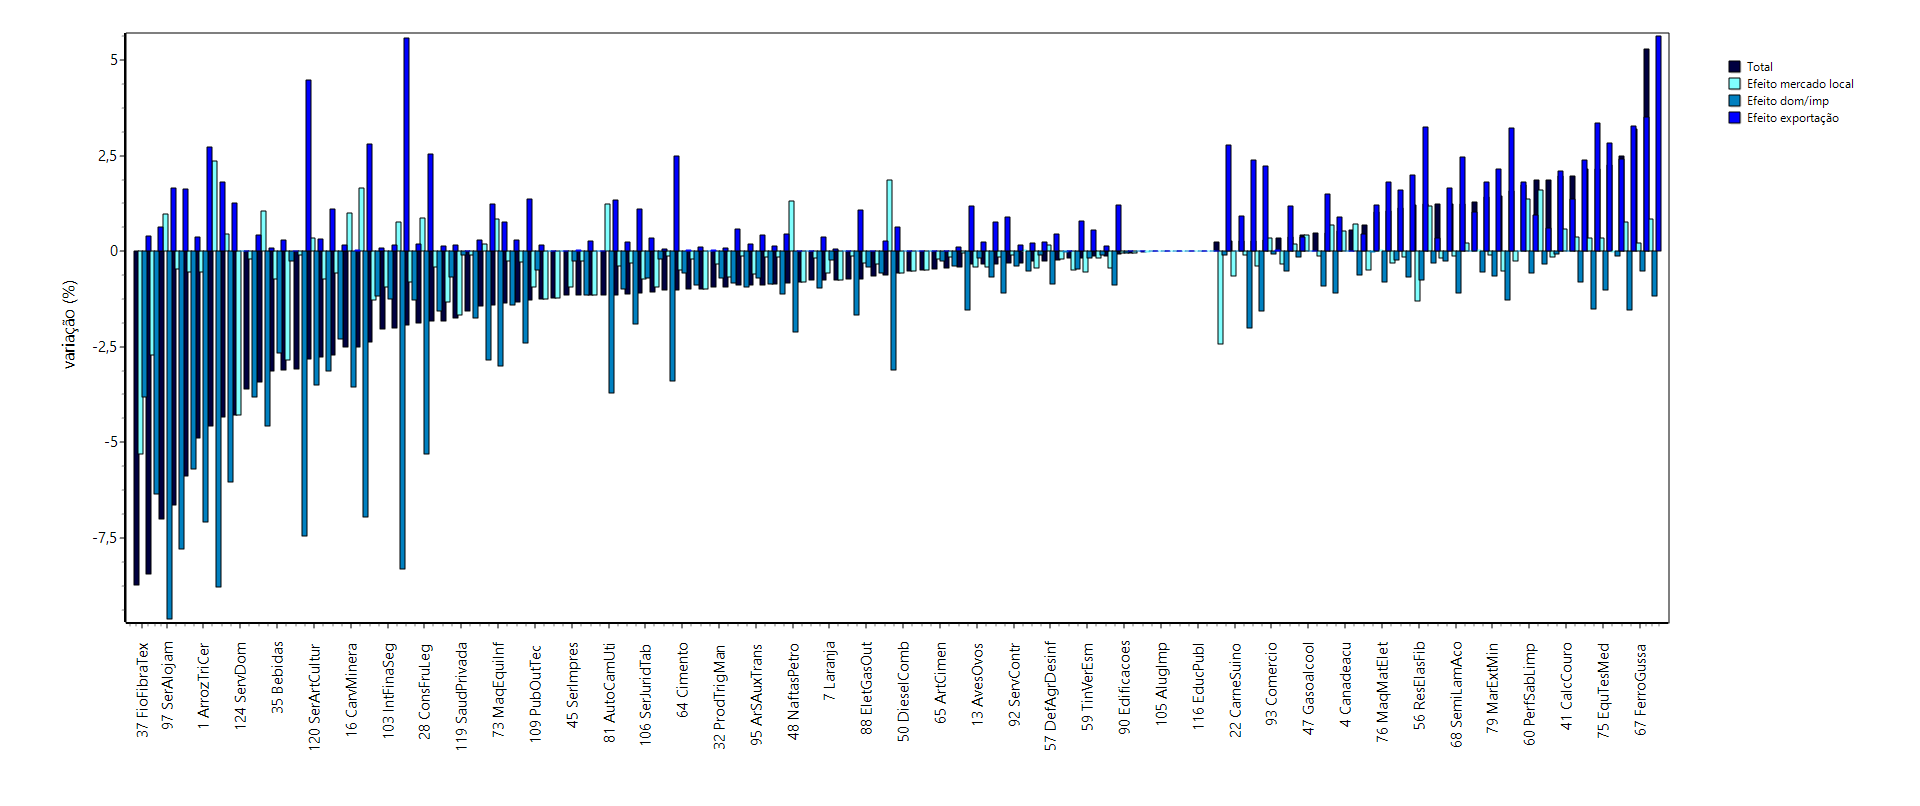
\includegraphics[width=\linewidth]{Imagens/006.ai}
		\footnotesize
		Fonte: elaboração própria (2024)
	\end{figure}
\end{landscape}


\subsection{Forma funcional} \label{subsec:forma_funcional}

Esta subseção apresenta o modelo de geração da renda familiar (\textit{Household Income Generation Model}) empregado para especificar a microssimulação comportamental utilizada neste trabalho, baseado em \textcite{bourguignon05}. Esse modelo consiste no conjunto de equações a seguir:

\begin{align}
	\Log \mathcal{w}_{mi}  &= \alpha_{g(mi)} + \beta_{g(mi)} \mathcal{x}_{mi} + \upsilon_{mi} \hspace{3cm} i = 1, \ldots, k_m \label{eq:renda} \\[0.5cm]
	IW_{mi}                &= \mathbbm{1} \left[\alpha_{h(mi)} + \beta_{h(mi)} z_{mi} + \mu_{mi} \right] \label{eq:ocm} \\[0.1cm]
	\text{Y}_{m}           &= \sum_{i = 1}^{k_{m}} \mathcal{w}_{mi} IW_{mi} + y_{0m} \label{eq:renda_media}
\end{align}

A equação~\eqref{eq:renda} apresenta os determinantes da renda $\mathcal{w}$ do indivíduo $\mathcal{i}$ da família $\mathcal{m}$ como função de suas características individuais, $\mathcal{x}$. A função $g()$ indica o segmento do mercado de trabalho\footnote{Por exemplo: gênero, habilidade ou área do domicílio. Para este trabalho, a função $g()$ representa o segmento de habilidade dos indivíduos -- não qualificado, semi-qualificado e qualificado.} ao qual pertence o indivíduo $\mathcal{i}$ da família $\mathcal{m}$.

A equação~\eqref{eq:ocm} representa a escolha ocupacional do indivíduo $\mathcal{i}$ da família $\mathcal{m}$. Todos os indivíduos são confrontados com uma escolha discreta: trabalhar ou não trabalhar. Desse modo, $IW_{mi}$ é uma variável \textit{dummy} na qual zero representa o indivíduo inativo e um, trabalhador assalariado, sendo função de suas características individuais e familiares, $z$. Isto implica que o modelo não atribui a todos os indivíduos uma escolha particular, mas dá as probabilidades individuais de estar numa condição e não na outra. Ou seja, o modelo gera uma distribuição de probabilidade sobre as duas diferentes alternativas \cite{colombo08}.

Seguindo a lógica da equação anterior, a função $h()$ indica o grupo demográfico\footnote{As características individuais, e seus coeficientes, podem variar de acordo com a posição do indivíduo na família.} ao qual pertence o indivíduo $\mathcal{i}$ da família $\mathcal{m}$. Por simplicidade, assume-se aqui que todos os assalariados têm jornadas integrais de trabalho.

A equação~\eqref{eq:renda_media} é uma identidade contábil que define o rendimento da família $Y_m$ como a soma da renda advinda do trabalho e de todos os outros rendimentos que não venham do mercado de trabalho, $y_{0m}$. A \textit{dummy} da escolha ocupacional garante que os salários que forem somados sejam apenas dos indivíduos realmente engajados no mercado de trabalho.

Ou seja, o modelo de geração da renda familiar define o rendimento total de uma dada família $\mathcal{m}$ como uma função das características observadas ($\mathcal{x_{mi}}$, $z_{mi}$) e não observadas ($\upsilon_{mi}$, $\mu_{mi}$) dos indivíduos e dos familiares. Essa função depende de dois blocos de parâmetros: 1- dos determinantes de renda ($\alpha_g$, $\beta_g$) para os segmentos do mercado de trabalho; e 2- da escolha ocupacional ($\alpha_h$, $\beta_h$) para os grupos sociodemográficos. Com essas informações, tem-se o modelo completo.


\subsection{Integração com o modelo EGC}\label{subsec:integracao}

O link entre um modelo EGC e uma microssimulação se dá pelos parâmetros. É a partir deles que os resultados do primeiro podem ser transmitidos para a o segundo. Ou seja, a integração macro-micro consiste em associar choques macroeconômicos e alterações em políticas simuladas no modelo EGC com alterações no conjunto de parâmetros do modelo de microssimulação.

O primeiro passo para a integração é criar a simulação de \textit{benchmarking}, necessária para se obter um conjunto inicial de parâmetros da microssimulação. A partir disso, o choque macroeconômico pauta a magnitude da variação desses parâmetros para que haja a integração entre os dois modelos.

Entretanto, essa associação deve ser feita de maneira consistente. Para o modelo de microssimulação proposto nesta dissertação, deve-se garantir: 1- variações nos rendimentos médios da microssimulação devem ser iguais às alterações na taxa salarial obtida com o modelo EGC; e 2- as mudanças no número de trabalhadores assalariados no modelo de microssimulação devem corresponder às observadas no modelo EGC \cite{bourguignon05, colombo08}.

Isso significa que o modelo EGC determina o nível de emprego da economia após a simulação e o modelo de microssimulação seleciona quais indivíduos entre as pessoas inativas têm a maior probabilidade de se ingressarem no mercado de trabalho -- supondo aumento do nível de emprego a partir do resultado do EGC. Ou quem, entre os trabalhadores assalariados, tem a menor probabilidade de estar empregado após a simulação -- supondo redução do nível de emprego. O indivíduo que ingresse no mercado ou seja realocado tem seu salário estimado pela equação dos determinantes de renda. 

Seja $E_G$ o nível de emprego no segmento G e $w_G$, o salário. A notação \^{} indica que é uma variável estimada a partir do modelo de geração da renda familiar. A consistência pode ser formalizada a partir deste conjunto de restrições \cite{bourguignon05}:

\begin{align}
	E_G &= \left\langle \sum_{mi}^{3} \mathbbm{1} \left[ \hat{\alpha}_{h(mi)} + \hat{\beta}_{h(mi)} z_{mi} + \hat{\mu}_{mi} \right] \right\rangle_{G} \label{eq:emprego_ag} \\
	\mathcal{w}_G &= \left\langle \sum_{mi}^{3} \text{Exp} \left( \hat{\alpha}_G + \hat{\beta}_G x_{mi} + \hat{\upsilon}_{mi} \right) \cdot \mathbbm{1} \left[ \hat{\alpha}_{h(mi)} + \hat{\beta}_{h(mi)} z_{mi} + \hat{\mu}_{mi} \right] \right\rangle_{G} \label{eq:renda_ag}
\end{align}

A equação~\eqref{eq:emprego_ag} representa a soma do nível de emprego assalariado para cada um dos segmentos do mercado de trabalho -- neste trabalho, às três categorias do fator trabalho: não qualificado, semi-qualificado e qualificado. A equação~\eqref{eq:renda_ag} representa a massa salarial para cada um dos segmentos do mercado de trabalho.

Supõe-se agora um choque exógeno do modelo EGC que altera as variáveis ($E_G$, $w_G$) para ($E_G^*$, $w_G^*$). Buscando garantir a consistência da integração macro-micro, deve-se encontrar um novo conjunto de parâmetros $C^*$ = ($\alpha_g^*$, $\beta_g^*$, $\alpha_h^*$, $\beta_h^*$) que mantenha a mesma validade do conjunto C = ($\alpha_g$, $\beta_g$, $\alpha_h$, $\beta_h$). 

Para isso, é necessário novas restrições. Há diversas maneiras de garantir a mesma validade para o conjunto $C^*$. A estratégia adotada neste trabalho segue a escolha de \textcite{bourguignon05} em restringir a variação apenas aos interceptos $a_g$ e $a_h$. A vantagem dessa estratégia é que implica em uma neutralidade nas mudanças feitas no que diz respeito às características individuais ou familiares. Ou seja, a alteração no intercepto $a_g$ gera uma mudança proporcional em todas as rendas do trabalho dentro do mesmo segmento, independentemente das características individuais e familiares -- desde que essas não sejam definidoras dos próprios segmentos.

Também há um semelhante argumento para os modelos de escolha discreta. De acordo com \textcite{bourguignon05}, uma mudança no intercepto $a_h$ implica na referida propriedade de neutralidade. A mudança relativa na probabilidade ex-ante de um indivíduo ter alguma ocupação depende apenas das probabilidades ex-ante iniciais das diversas escolhas ocupacionais, e não das características individuais.

Portanto, o link entre os modelos EGC e de geração da renda familiar é obtido através da resolução do seguinte sistema de equações:

\begin{align}
	E_G^* &= \left\langle \sum_{mi}^{3} \mathbbm{1} \left[ \hat{\alpha}_{h(mi)}^* + \hat{\beta}_{h(mi)}^* z_{mi} + \hat{\mu}_{mi} \right] \right\rangle_{G} \label{eq:emprego_ag*} \\
	\mathcal{w}_G^* &= \left\langle \sum_{mi}^{3} \text{Exp} \left( \hat{\alpha}_G^* + \hat{\beta}_G x_{mi} + \hat{\upsilon}_{mi} \right) \cdot \mathbbm{1} \left[ \hat{\alpha}_{h(mi)}^* + \hat{\beta}_{h(mi)} z_{mi} + \hat{\mu}_{mi} \right] \right\rangle_{G} \label{eq:renda_ag}
\end{align}

Uma vez solucionado esse sistema de equações, deve-se calcular a nova renda de cada família da amostra, conforme indicam as equações~\eqref{eq:renda} --~\eqref{eq:renda_media}, usando o conjunto $C^*$. Depois, resta por analisar o novo cenário da distribuição de renda e os efeitos dos novos parâmetros.


\subsection{Abordagem empírica} \label{subsec:abordagem_empirica}

Uma vez definida a forma funcional da microssimulação e o processo de integração com o modelo EGC, deve-se estimar o modelo de geração da renda familiar. Para este trabalho, optou-se por utilizar a Correção de Heckman para a equação~\eqref{eq:renda} dos determinantes de renda \cite{heckman79}. Desse modo, pode-se corrigir um viés de seleção implícito a uma regressão salarial\footnote{Só é observado uma renda do trabalho positiva para os indivíduos que estão empregados no momento da pesquisa amostral.}.

A Correção de Heckman é dividida em duas etapas: na primeira, executa-se um modelo de escolha discreta, que tem o objetivo de estimar a probabilidade ingressar no mercado de trabalho para se poder calcular a Inversa de Mills. A equação~\eqref{eq:step1} apresenta a especificação dessa primeira etapa.

\begin{align}
	\textbf{Trab}_{g(mi)}        &= \mathbf{X}_{g(mi)} \ \boldsymbol{\hat{\beta}} + \boldsymbol{\varepsilon}_{g(mi)} \label{eq:step1} \\
	\boldsymbol{\Lambda}_{g(mi)} &= \frac{\phi(x)}{1 - \Phi(x)} \label{eq:mills}
\end{align}

Na qual $\text{Trab}_{g(mi)}$ é uma variável \textit{dummy} de participação no mercado de trabalho. $\mathbf{X}_{g(mi)}$ é uma matriz formada pelas seguintes variáveis independentes: anos de estudo, experiência potencial e experiência potencial quadrática, renda domiciliar per capita. Também é formada por variáveis de controle para gênero, raça, situação do domicílio, setor, unidade federativa e características do chefe de família -- como idade, sexo, anos de estudo, se é casado e o número de filhos.

A equação~\eqref{eq:mills} exibe o cálculo da Inversa de Mills, no qual $\phi(x)$ representa função de densidade normal padrão, e $\Phi(x)$ a função de distribuição cumulativa normal padrão. Seu valor é usado na segunda etapa da Correção para corrigir o viés de seleção. A equação~\eqref{eq:step2} apresenta sua especificação.

\begin{align}
	\mathbf{\Log \mathcal{w}}_{g(mi)} = \mathbf{Z}_{g(mi)} \ \boldsymbol{\hat{\beta}} + \boldsymbol{\Lambda}_{g(mi)} + \boldsymbol{\varepsilon}_{g(mi)} \label{eq:step2}
\end{align}

Na qual $\mathbf{\Log \mathcal{w}}_{g(mi)}$ é o logaritmo da renda-hora do indivíduo $i$ da família $m$. $\mathbf{Z}_{g(mi)}$ é uma matriz de variáveis independentes que contém: anos de estudo, experiência potencial e experiência potencial quadrática, situação do domicílio e variáveis de controle por gênero, raça, setor e unidade federativa. Como citado anteriormente, $\boldsymbol{\Lambda}_{g(mi)}$ representa a Inversa de Mills.

Para estimar a equação~\eqref{eq:ocm} da escolha ocupacional, optou-se por um modelo de regressão logística, assumindo que o termo residual está distribuído de acordo com a Lei Exponencial Dupla -- ou Distribuição de Laplace \cite{bourguignon05}. Segue abaixo sua especificação:

\begin{align}
	\textbf{Trab}_{g(mi)} &= \mathbf{X}_{g(mi)} \ \boldsymbol{\hat{\beta}} + \boldsymbol{\varepsilon}_{g(mi)} \label{eq:logit}
\end{align}

Na qual $\mathbf{X}_{g(mi)}$ é a mesma matriz de variáveis independentes utilizada na primeira etapa da Correção de Heckman. Para todas as equações estimadas, $\boldsymbol{\varepsilon}_{g(mi)}$ representa o termo de erro, também chamado de resíduo, que captura fatores não observados, erros de mensuração e outras influências que não são explicadas pelas variáveis incluídas no modelo.. A tabela com a descrição completa de todas as variáveis independentes está disponível no Apêndice~\ref{ap:a}.


\subsection{Base de dados} \label{subsec:dados_microssimulacao}

Para estimar o modelo de geração da renda familiar, optou-se por utilizar os dados \citetitle*{pnad} referente ao ano de 2015. Essa base contém informações	sobre os domicílios brasileiros e as características pessoais e socioeconômicas de seus indivíduos por setor produtivo e região geográfica, totalizando cerca de 356.904 observações. Sua escolha se baseia na necessidade de garantir compatibilidade entre os resultados dos dois modelos utilizados neste trabalho. Ao usar a PNAD 2015 para calibrar o modelo ORANIG-BR e substanciar o modelo de geração de renda familiar, abre-se espaço para que os resultados sejam compatíveis e, por conseguinte, possam dialogar entre si.


